% arara: pdflatex
% arara: pdflatex
% arara: pdflatex

% options:
% thesis=B bachelor's thesis
% thesis=M master's thesis
% czech thesis in Czech language
% slovak thesis in Slovak language
% english thesis in English language
% hidelinks remove colour boxes around hyperlinks

\documentclass[thesis=M,czech]{FITthesis}[2019/12/23]
\makeatletter\AtBeginDocument{\let\@elt\relax}\makeatother

\usepackage[utf8]{inputenc} % LaTeX source encoded as UTF-8

\usepackage{amsmath} %advanced maths
\usepackage{amssymb} %additional math symbols

\usepackage{graphicx}
\graphicspath{ {./img/} }

\usepackage{dirtree} %directory tree visualisation
\RequirePackage{pdfpages}

% % list of acronyms
% \usepackage[acronym,nonumberlist,toc,numberedsection=autolabel]{glossaries}
% \iflanguage{czech}{\renewcommand*{\acronymname}{Seznam pou{\v z}it{\' y}ch zkratek}}{}
% \makeglossaries

\newcommand{\tg}{\mathop{\mathrm{tg}}} %cesky tangens
\newcommand{\cotg}{\mathop{\mathrm{cotg}}} %cesky cotangens

% % % % % % % % % % % % % % % % % % % % % % % % % % % % % % 
% ODTUD DAL VSE ZMENTE
% % % % % % % % % % % % % % % % % % % % % % % % % % % % % % 

\department{Katedra softwarového inženýrství}
\title{Srovnání REST, GraphQL a gRPC API v~Node.js}
\authorGN{Tomáš} %(křestní) jméno (jména) autora
\authorFN{Buňata} %příjmení autora
\authorWithDegrees{Bc. Tomáš Buňata} %jméno autora včetně současných akademických titulů
\author{Tomáš Buňata} %jméno autora bez akademických titulů
\supervisor{Ing. Lukáš Loukota}
\acknowledgements{Doplňte, máte-li komu a za co děkovat. V~opačném případě úplně odstraňte tento příkaz.}
\abstractCS{V~několika větách shrňte obsah a přínos této práce v~češtině. Po přečtení abstraktu by se čtenář měl mít čtenář dost informací pro rozhodnutí, zda chce Vaši práci číst.}
\abstractEN{Sem doplňte ekvivalent abstraktu Vaší práce v~angličtině.}
\placeForDeclarationOfAuthenticity{V~Praze}
\declarationOfAuthenticityOption{4} %volba Prohlášení (číslo 1-6)
\keywordsCS{Nahraďte seznamem klíčových slov v češtině oddělených čárkou.}
\keywordsEN{Nahraďte seznamem klíčových slov v angličtině oddělených čárkou.}
% \website{http://site.example/thesis} %volitelná URL práce, objeví se v tiráži - úplně odstraňte, nemáte-li URL práce

\begin{document}

% \newacronym{CVUT}{{\v C}VUT}{{\v C}esk{\' e} vysok{\' e} u{\v c}en{\' i} technick{\' e} v Praze}
% \newacronym{FIT}{FIT}{Fakulta informa{\v c}n{\' i}ch technologi{\' i}}

\begin{introduction}
Webové aplikace jsou každodenní součástí našeho života. Setkáváme se s nimi při čtení ranních zpráv, komunikaci se svými přáteli nebo spravování financí přes internetové bankovnictví.
Architektura webových aplikací se dá rozdělit na dvě hlavní části: frontend (část se kterou interaguje uživatel v prohlížeči) a backend (serverová část, která slouží k ukládání a  manipulaci s daty). V této práci se věnuji té druhé části - konkrétně backendovým technologiím zprostředkovávající komunikaci mezi serverem a klientem.
Vzhledem k tomu, že webové technologie se velmi rychle vyvíjejí a posouvají vpřed, vývojáři velmi často narážejí na otázku výběru správné technologie pro svůj projekt. V této práci se pokusím na tuto otázku odpovědět. Porovnám mezi sebou následující: REST, GraphQL a gRPC.

REST je z těchto technologií nejstarší a v současnosti také nejpopulárnější. Princip RESTu je takový, že každá entita je identifikována unikátním URI a pomocí HTTP metod je s těmito entitami manipulováno.
GraphQL vzniklo přibližně o deset let později a funguje zcela na odlišném principu - vystavuje jediný endpoint, na který se poté dotazujeme speciálním jazykem, který strukturou velmi přípomína JSON.
gRPC je z těchto technologií nejmladší a jedná se o open source implementaci RPC (volání vzdálené procedury) od společnosti Google.

S každou z těchto technologií implementuji aplikační rozhraní pro eshop a následně je porovnám ze stránek uživatelské zkušenosti, podpory vývojářů a míry schopnosti zvládat zátěž.
V teoretické části práce se budu věnovat představení těchto technologií. Poté se budu věnovat požadavkům na návrh backendu aplikace, na kterém tyto technologie budou demonstrovány. Další část se bude věnovat výběru databázového systému a dalších technologií potřebných pro správné fungování aplikace.
V praktické části se budu nejdříve věnovat implementaci jednotlivých backendů, včetně otestování jejich správné funkčnosti, a poté otestuji jejich výkon zátěžovými testy. Poslední část se bude věnovat věnovat samotnému srovnání těchto technologií.

\end{introduction}

\chapter{Cíl práce}
Cílem práce je návrh a implementace  tří shodných API v REST, GraphQL a gRPC, která budou realizovat typické operace, které využívají eshopy - např. vytvoření účtu zákazníka, listování produktů nebo vytvoření objednávky. Tato API budou implementována nad Node.js.

Teoretická část se zabývá samotným návrhem API, kde jsou prozkoumány různé služby, které by měly být integrované do systému. Návrh vychází z typických operací potřebných pro chod eshopu. V této části budou také popsány použité technologie.

Cílem praktické části je implementace je navázat na předchozí část implementací navrženého API. Bude ukázány klíčové implementační kroky, které jsou potřeba pro realizaci API v daných technologií. Součástí implementace je také napsání testů, které ověří funkčnost vytvořených systémů.\\
Dále zde bude popsána metodologie porovnání (dokumentace, rychlost vývoje, výkonnostní testování, ...) a na základě této metodologie budou tyto technologie porovnány.



\chapter{Analýza a návrh}
Před tím, než se začneme věnovat návrhu a implementaci API, je v hodné si nejdříve vysvětlit co znamená pojem API a následně představím co to je REST, GraphQL a gRPC. Současně také popíšu jaké knihovny jsem si vybral pro jejich implementaci. A poté představím samotný návrh API, které bude implementováno v praktické části.

\section{API}
Zkratka API označuje rozhraní pro programování aplikací. Jedná se o velmi důležitou součást vývoje, protože definuje způsob jak mezi sebou budou jednotlivé aplikace (nebo komponenty v rámci jedné aplikace) komunikovat. Dalo by se říci, že představuje smlouvu, kterou obě strany musí dodržet abz spolu mohli komunikovat\\
API se skládá ze dvou částí: 
\begin{itemize}
    \item Technické specifikace, která popisuje možnosti komunikace - metody, které API vystavuje, vstupní data...
    \item Softwarového rozhraní, které tuto specifikaci implementuje
\end{itemize}

API se dále mohou dělit podle dostupnosti na soukromá, partnerská nebo otevřená. Soukromá API se používají výhradně v rámci jedné organizace. Ikdyž aplikace, které tato API využívají mohou být veřejně dostupné, samotné rozhraní není.\\
Partnerská APi jsou sdílená s business partnery a slouží hlavně k integraci systémů mezi partnery a společností, která poskytuje přístup k API.\\
Otevřená API jsou volně dostupná všem vývojářům a je možné je využívat bez explicitního souhlasu poskytovatele těchto rozhraní nebo bez licenčních poplatků. Poplatky mohou být účtované za informace dostupné za rozhraním, ale dokumentace  a testovací data musí být veřejně dostupná.

Aplikační programovací rozhraní jdou také dělit podle způsobu použití. Může se jednat třeba o databázové API, které umožnuje komunikaci mezi aplikací a databázovým systémem, nebo API operačního systému, které definuje jak programy mohou využívat zdroje a služby operačního systému.\\
Nejběžnější, a z pohledu této práce také nejzajímavější, jsou však webová aplikační rozhraní, která poskytují data a funkcionality mezi webovými systémy reprezentující architekturu klient-server. Tato API typicky doručují požadavky z webových aplikací a odpovědi ze serverů prostřednictvím protokolu HTTP. Mezi jeden z nejpopulárnějších typů webových aplikační rozhraní patří REST, ikdyž v poslední době jeho popularita začíná pomalu klesat, viz obrázek \ref{google_trends_img} \cite{google-trends}.

\begin{figure}[h]
    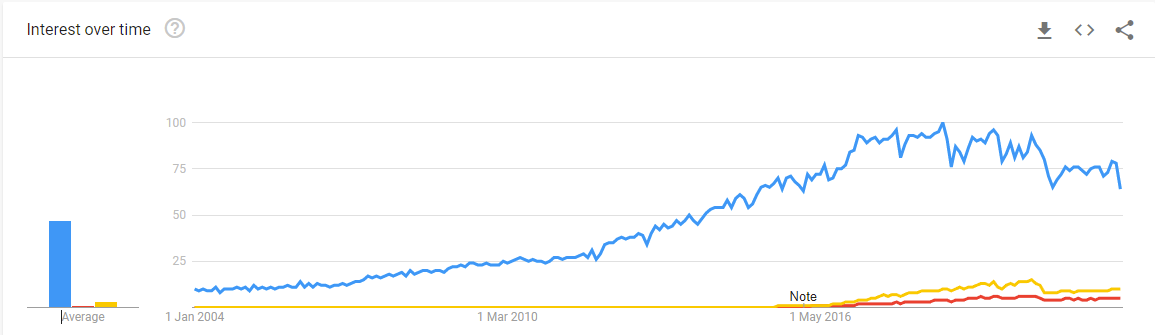
\includegraphics[width=\linewidth]{img/interest_trend.png}
    \caption{Google Trends: REST (modrá), GraphQL (žlutá) a gRPC (červená)}
	\label{google_trends_img}
\end{figure}

\section{REST}
REST je velmi oblíbený architektonický styl pro tvorbu API, který vyniká svou jednoduchostí a čitelností. Na rozdíl např. od gRPC není orientován procedurálně, ale datově.\\
Zkratka REST vyjadřuje pojem representational state transfer a v roce 2000 ji zavedl Roy Fielding ve své dizertační práci \cite{fielding00}. Než si vysvětlíme, jaké požadavkz musí REST API splňovat, je potřeba vysvětlit co to je zdroj.\\
Jakákoli informace, kterou lze pojmenovat, může být zdrojem. Může to být například obrázek, dočasná služba nebo kolekce jiných zdrojů. Stav zdroje v čase nazýváme reprezentace zdroje. Skládá se ze tří částí - dat, metadat popisující tato data a hypermedia odkazů, která pomáhají klientům s přechodem do dalšho požadovaného stavu.

Aby aplikační rozhraní mohlo být nazýváno RESTful, je potřeba aby splňovalo šest architektonických omezení \cite{restful_api}:

\subsection{Uniform Interface}
Aplikováním principu generality na rozhraní komponenty můžeme zjednodušit architekturu celého systému. Tomu pomáhá několik omezení.
\begin{itemize}
    \item \textbf{Identifikace zdrojů} - Rozhraní musí jednoznačně identifikovat každý zdroj, který je použit v interakci mezi klientem a serverem
    \item \textbf{Manipulace se zdroji} skrz jejich reprezentaci - Zdroje v odpovědi serveru by měly mít jednotnou reprezentaci. Konzumenti API by pak měli použít tyto reprezentace k modifikování stavu zdrojů.
    \item \textbf{Samopopisující se zprávy} - Každá reprezentace zdroje by měla obsahovat dostatek informací aby bylo jasné jak ji zpracovat. Měla by také obsahovat jaké další možné operace může klient se zdrojem provádět.
    \item \textbf{Hypermedia jako aplikační stav} - Klient by měl mít pouze počáteční URI aplikace. Klientská aplikace by poté měla řídit veškeré interakce pomocí hyperlinků - serverová odpověď obsahuje seznam dostupných operací.
\end{itemize}

\subsection{Client-server}
Návrhový vzor klient-server vynucuje oddělení zodpovědností, což pomáhá tomu aby se klientské a serverové komponenty mohly vyvíjet nezávisle na sobě. Zatímco se server a klient vyvíjí, je potřeba dávat pozor, aby rozhraní mezi nimi nebylo porušeno.
Oddělením uživatelského rozhraní (klienta) a manipulaci s daty (serveru) umožníme nezávislost uživatelského rozhraní na konkrétní platformě a zároveň zlepšíme škálovatelnost serveru zjednodušením jeho komponent. Servery nebo klienti mohou být také nahrazeny, pokud nedojde ke změně rozhraní

\subsection{Stateless}
Bezestavovost požaduje, že každý požadavek z klienta na server musí obsahovat všechny dostupné informace potřebné k jeho zpracování. Server nemůže využívat žádných uložených informací z předchozích interakcí - chová se jako kdybz každý požadavek byl úplně nový. Z toho vyplývá, že klient je zodpovědný za udržování aplikačního stavu, pokud to je potřeba.

\subsection{Cacheable}
Toto omezení požaduje, že každá odpověď serveru by se měla označit jako cachovatelná nebo necachovatelná. Pokud je cachovatelná, klient má po omezenou dobu právo tyto informace přepoužít v dalších požadavcích

\subsection{Layered system}
REST umožnuje využití vrstvené architektury, kde například server A obsahuje API, na serveru B se ukládají data a na serveru C se autentizují požadavky. Klient nemůže zjistit, jestli je ke konkrétnímu serveru připojen přímo nebo přes prostřeníka.

\subsection{Code on demand - volitelné}
Umožnění rozšíření funkcionality klienta stažením a spuštěním kódu ve formě appletů nebo skriptů ze serveru. Výsledkem je zjednodušení klienta, který nemusí obsahovat tolik předinstalovaných funkcí.

\subsection{HTTP}
Pro přenos dat mezi klientem a servrem se nejčastěji používá protokol HTTP, ikdyž REST není vázaný na tento protokol. Protože ale se tato práce zabývá pouze webovými API, budu se v této práci věnovat pouze přenosu pomocí HTTP.
HTTP definuje množinu metod, které slouží k indikaci jakou akci chceme se zdrojem provést. Tyto metody se také označují jako \textit{HTTP verbs} \cite{http_metods}

\begin{itemize}
    \item \textbf{GET} - slouží k získání reprezentace daného zdroje. Měla by být použita pouze k získávání informací.
    \item \textbf{HEAD} - slouží k získání stejné odpovědi jako \textbf{GET}, ale bez těla odpovědi.
    \item \textbf{POST} - slouží k odeslání entity k danému zdroji, která často způsobí změnu stavu nebo side-effect na serveru.
    \item \textbf{PUT} - tato meto nahradí všechny současné reprezentace cílového zdroje za obsah požadavku
    \item \textbf{DELETE} - slouží ke smazání cílového zdroje.
    \item \textbf{PATCH} - slouží k částečné změně cílového zdroje
\end{itemize}

Metody, které nemění stav serveru označujeme jako bezpečné. Jedná se hlavně o GET a HEAD. V praxi ale bežně není možné tyto metody na straně serveru implementovat tak, aby neměnily vůbec žádný stav - může například dojít k zalogování metody nebo obnovení cache.

Další kategorie jsou idempotetní metody. Idempotence znamená, že pokud klient provede několik shodných požadavků, všechny budou mít stejný výsledek. Jedná se hlavne o GET, HEAD, PUT a DELETE. To ale neznamená, že server musí na každý požadavek odpovědět stejně.


\subsubsection*{Stavové kódy}
HTTP taktéž definuje stavové kódy odpovědí. Tyto kódy se v REST api využívají k informování klienta o výsledku prováděné operace. Tyto kódy se dělí do pěti kategorií, které se od sebe liší prvním číslem. Kódy s začínající číslem 100 jsou informační - komunikují informace na úrovni transportního protokolu \cite{http_codes}. Kódy začínající číslem 200 informují o úspěšném zpracování požadavku. Kódy s číslem 300 značí, že je potřeba dodatečná akce od klienta. Číslo 400 označuje chybový stav na straně klienta. Poslední jsou pak kódy s číslem 500, které označují chybu na straně serveru. Nejčastěji se setkáme s následujícími kódy:
\begin{itemize}
    \item 200 OK - Požadavek proběhl v pořádku. Na rozdíl od kódu 204 by odpověď měla obsahovat i data, a je závislá na použité metodě. Například pro GET by se mělo jednat o reprezentaci zdroje, zatímco pro POST se může jednat o výsledek operace. %todo%
    \item 201 Created - Požadavek proběhl v pořádku a jeho výsledkem je vytvoření zdroje. Typicky se jedná o vytvoření zdroje uvnitř kolekce pomocí POST metody.
    \item 204 No Content - Server naplnil požadavek, ale není potřeba vrátit žádnou hodnotu. Například při operaci DELETE, kdy mažeme zdroj z kolekce. Tělo odpovědi nesmí obsahovat žádná data.
    \item 400 Bad Request - Požadavek je pro server nečitelný. Jedná se o obecný chybový kód, který se použije pokud žádný jiný není vhodný. Může se například jednat o špatný formát požadavku. Klient by stejný požadavek neměl opakovat beze změny.
    \item 401 Unauthorized - Klient není ověřen. Požadavek může být opakován s doplněnými informacemi o oveření.
    \item 403 Forbidden - Klient nemá dostatečná práva. Narozdíl od 401, identita klienta je známa.
    \item 404 Not Found - Server nenašel požadovaný zdroj.
    \item 405 Method Not Allowed - Klient použil metodu, kterou daný zdroj nepodporuje. Odpověď musí obsahovat hlavičku s výčtem podporovaných metod.
    \item 500 Internal Server Error - Server narazil na neočekávanou chybu při zpracování požadavku. Jedná se o obecný chybový kód. Nikdy se nejedná o chybu klienta a dává smysl stejný požadavek opakovat s očekáváním jiné odpovědi.
    \item 503 Service Unavailable - Server není připravený zpracovat požadavek.
\end{itemize}

\section{GraphQL}
GraphQL bylo vytvořeno společností Facebook v roce 2012. Hlavním důvodem jeho vzniku byla narůstající potřeba API pro získávání dat, které bude dostatečně silné a zároveň bude jednoduché na používání. V roce 2015 pak bylo GraphQL zpřístupněno jako opensource \cite{graphql_fb}. Od této doby vznikla spousta implementací v různých jazycích jako je Javascript, Java, Python a mnoha dalších.

\subsection{Základní vlastnosti}
\subsubsection*{Definuje strukturu dat}
První věcí, kterou si na GraphQL můžeme všimout je to, že struktura dat posílaných na server se velmi podobá struktuře dat vrácených v odpovědi, viz obrázek \ref{graphql-query}. To přispívá ke zjednošení psaní dotazů - pokud víme jaká data server potřebuje - a také víme jaký formát dat očekávat. To je jedna z velkých výhod GraphQL, klient si určuje formát dat posílaných ze serveru a má tak přizpůsobená data pro své požadavky.

\begin{figure}[h]
    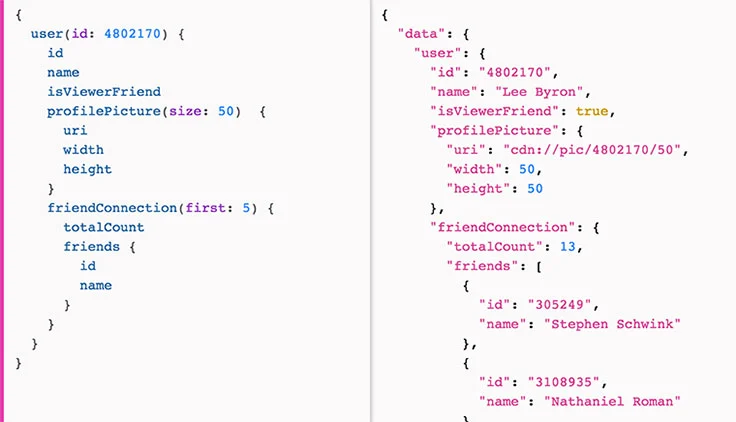
\includegraphics[width=\linewidth]{img/graphql-query.png}
    \caption{Příklad GraphQL dotazu a odpovědi \cite{graphql_query_img}}
	\label{graphql-query}
\end{figure}

\subsubsection*{Hierarchický}
Dalším důležitým apektem GraphQL je jeho hierarchičnost. Přirozeně totiž sleduje vztahy mezi objekty a oproti RESTu tak dovoluje vyhnout se několikanásobnému volání API pro získání dat souvisejících objektů.

\subsubsection*{Silně typový}
Každý GraphQL server definuje typový systém, který je specifický pro aplikaci.
Každá úroveň GraphQL dotazu odpovídá určitému typu a každý typ má definovanou množinu atributů, které obsahuje. Toto umožňuje validaci dotazů ještě před odesláním na server a zobrazování relevantních chybových hlášek.

\subsection*{Protokol, ne úložiště}
Každému atributu v GraphQL na serveru odpovídá nějaká funkce. Pokud už máme existující logiku aplikace společně s úložištěm, můžeme toto všechno na GraphQL napojit.

\subsection*{Introspekce}
Díky typovému systému máme možnost prozkoumávat schéma a zjistit dostupné \textit{queries}, \textit{mutace} nebo \textit{subscriptions}. Schéma také slouží jako smlouva mezi frontendem a backendem definující jak spolu budou komunikovat.
Introspekce také vytváří platformu pro různé nástroje - od generování kódu po tvorbu dokumentace.

\subsection*{GraphQl dotaz}
%img: https://www.apollographql.com/blog/static/5d820420290da80546e26d7c966b1d74/Untitled-1.png%
GraphQL dotaz je řetězec, který je poslán na server, vyhodnocen a jeho výsledek je zaslán ve formátu JSON zpátky klientovi.

\subsubsection*{GraphQL query}



>>>>>>> feat: add rest description

\section{gRPC}

\section{Node.js }
\section{Návrh}
Aby srovnání co nejvíce odpovídalo realitě, vybral jsem si jako vzor pro API, které budu implementovat, eshop. Je to typický příklad, se kterým se vývojář může setkat při své práci a zároveň je tento vzor dost obecný na to, aby si čtenář mohl jednoduše převést na jiný. Pro popis api jsem zvolil specifikaci OpenAPI.

\subsection{OpenAPI}
OpenAPI 

\chapter{}

\chapter{Realizace}

\chapter{Testování}

\chapter{Závěrečné srovnání}

\begin{conclusion}
	%sem napište závěr Vaší práce
\end{conclusion}

\bibliographystyle{csn690}
\bibliography{mybibliographyfile}

\appendix

\chapter{Seznam použitých zkratek}
% \printglossaries
\begin{description}
	\item[REST] Representational state transfer
	\item[RPC] Remote procedure call
	\item[XML] Extensible markup language
\end{description}


% % % % % % % % % % % % % % % % % % % % % % % % % % % % 
% % Tuto kapitolu z výsledné práce ODSTRAŇTE.
% % % % % % % % % % % % % % % % % % % % % % % % % % % % 
% 
% \chapter{Návod k~použití této šablony}
% 
% Tento dokument slouží jako základ pro napsání závěrečné práce na Fakultě informačních technologií ČVUT v~Praze.
% 
% \section{Výběr základu}
% 
% Vyberte si šablonu podle druhu práce (bakalářská, diplomová), jazyka (čeština, angličtina) a kódování (ASCII, \mbox{UTF-8}, \mbox{ISO-8859-2} neboli latin2 a nebo \mbox{Windows-1250}). 
% 
% V~české variantě naleznete šablony v~souborech pojmenovaných ve formátu práce\_kódování.tex. Typ může být:
% \begin{description}
% 	\item[BP] bakalářská práce,
% 	\item[DP] diplomová (magisterská) práce.
% \end{description}
% Kódování, ve kterém chcete psát, může být:
% \begin{description}
% 	\item[UTF-8] kódování Unicode,
% 	\item[ISO-8859-2] latin2,
% 	\item[Windows-1250] znaková sada 1250 Windows.
% \end{description}
% V~případě nejistoty ohledně kódování doporučujeme následující postup:
% \begin{enumerate}
% 	\item Otevřete šablony pro kódování UTF-8 v~editoru prostého textu, který chcete pro psaní práce použít -- pokud můžete texty s~diakritikou normálně přečíst, použijte tuto šablonu.
% 	\item V~opačném případě postupujte dále podle toho, jaký operační systém používáte:
% 	\begin{itemize}
% 		\item v~případě Windows použijte šablonu pro kódování \mbox{Windows-1250},
% 		\item jinak zkuste použít šablonu pro kódování \mbox{ISO-8859-2}.
% 	\end{itemize}
% \end{enumerate}
% 
% 
% V~anglické variantě jsou šablony pojmenované podle typu práce, možnosti jsou:
% \begin{description}
% 	\item[bachelors] bakalářská práce,
% 	\item[masters] diplomová (magisterská) práce.
% \end{description}
% 
% \section{Použití šablony}
% 
% Šablona je určena pro zpracování systémem \LaTeXe{}. Text je možné psát v~textovém editoru jako prostý text, lze však také využít specializovaný editor pro \LaTeX{}, např. Kile.
% 
% Pro získání tisknutelného výstupu z~takto vytvořeného souboru použijte příkaz \verb|pdflatex|, kterému předáte cestu k~souboru jako parametr. Vhodný editor pro \LaTeX{} toto udělá za Vás. \verb|pdfcslatex| ani \verb|cslatex| \emph{nebudou} s~těmito šablonami fungovat.
% 
% Více informací o~použití systému \LaTeX{} najdete např. v~\cite{wikilatex}.
% 
% \subsection{Typografie}
% 
% Při psaní dodržujte typografické konvence zvoleného jazyka. České \uv{uvozovky} zapisujte použitím příkazu \verb|\uv|, kterému v~parametru předáte text, jenž má být v~uvozovkách. Anglické otevírací uvozovky se v~\LaTeX{}u zadávají jako dva zpětné apostrofy, uzavírací uvozovky jako dva apostrofy. Často chybně uváděný symbol "{} (palce) nemá s~uvozovkami nic společného.
% 
% Dále je třeba zabránit zalomení řádky mezi některými slovy, v~češtině např. za jednopísmennými předložkami a spojkami (vyjma \uv{a}). To docílíte vložením pružné nezalomitelné mezery -- znakem \texttt{\textasciitilde}. V~tomto případě to není třeba dělat ručně, lze použít program \verb|vlna|.
% 
% Více o~typografii viz \cite{kobltypo}.
% 
% \subsection{Obrázky}
% 
% Pro umožnění vkládání obrázků je vhodné použít balíček \verb|graphicx|, samotné vložení se provede příkazem \verb|\includegraphics|. Takto je možné vkládat obrázky ve formátu PDF, PNG a JPEG jestliže používáte pdf\LaTeX{} nebo ve formátu EPS jestliže používáte \LaTeX{}. Doporučujeme preferovat vektorové obrázky před rastrovými (vyjma fotografií).
% 
% \subsubsection{Získání vhodného formátu}
% 
% Pro získání vektorových formátů PDF nebo EPS z~jiných lze použít některý z~vektorových grafických editorů. Pro převod rastrového obrázku na vektorový lze použít rasterizaci, kterou mnohé editory zvládají (např. Inkscape). Pro konverze lze použít též nástroje pro dávkové zpracování běžně dodávané s~\LaTeX{}em, např. \verb|epstopdf|.
% 
% \subsubsection{Plovoucí prostředí}
% 
% Příkazem \verb|\includegraphics| lze obrázky vkládat přímo, doporučujeme však použít plovoucí prostředí, konkrétně \verb|figure|. Například obrázek \ref{fig:float} byl vložen tímto způsobem. Vůbec přitom nevadí, když je obrázek umístěn jinde, než bylo původně zamýšleno -- je tomu tak hlavně kvůli dodržení typografických konvencí. Namísto vynucování konkrétní pozice obrázku doporučujeme používat odkazování z~textu (dvojice příkazů \verb|\label| a \verb|\ref|).
% 
% \begin{figure}\centering
% 	
\includegraphics[width=0.5\textwidth, angle=30]{cvut-logo-bw}
% 	\caption[Příklad obrázku]{Ukázkový obrázek v~plovoucím prostředí}\label{fig:float}
% \end{figure}
% 
% \subsubsection{Verze obrázků}
% 
% % Gnuplot BW i barevně
% Může se hodit mít více verzí stejného obrázku, např. pro barevný či černobílý tisk a nebo pro prezentaci. S~pomocí některých nástrojů na generování grafiky je to snadné.
% 
% Máte-li například graf vytvořený v programu Gnuplot, můžete jeho černobílou variantu (viz obr. \ref{fig:gnuplot-bw}) vytvořit parametrem \verb|monochrome dashed| příkazu \verb|set term|. Barevnou variantu (viz obr. \ref{fig:gnuplot-col}) vhodnou na prezentace lze vytvořit parametrem \verb|colour solid|.
% 
% \begin{figure}\centering
% 	\includegraphics{gnuplot-bw}
% 	\caption{Černobílá varianta obrázku generovaného programem Gnuplot}\label{fig:gnuplot-bw}
% \end{figure}
% 
% \begin{figure}\centering
% 	\includegraphics{gnuplot-col}
% 	\caption{Barevná varianta obrázku generovaného programem Gnuplot}\label{fig:gnuplot-col}
% \end{figure}
% 
% 
% \subsection{Tabulky}
% 
% Tabulky lze zadávat různě, např. v~prostředí \verb|tabular|, avšak pro jejich vkládání platí to samé, co pro obrázky -- použijte plovoucí prostředí, v~tomto případě \verb|table|. Například tabulka \ref{tab:matematika} byla vložena tímto způsobem.
% 
% \begin{table}\centering
% 	\caption[Příklad tabulky]{Zadávání matematiky}\label{tab:matematika}
% 	\begin{tabular}{|l|l|c|c|}\hline
% 		Typ		& Prostředí		& \LaTeX{}ovská zkratka	& \TeX{}ovská zkratka	\tabularnewline \hline \hline
% 		Text		& \verb|math|		& \verb|\(...\)|	& \verb|$...$|		\tabularnewline \hline
% 		Displayed	& \verb|displaymath|	& \verb|\[...\]|	& \verb|$$...$$|	\tabularnewline \hline
% 	\end{tabular}
% \end{table}
% 
% % % % % % % % % % % % % % % % % % % % % % % % % % 

\chapter{Obsah přiloženého CD}

%upravte podle skutecnosti

% \begin{figure}
% 	\dirtree{
% 		.1 readme.txt\DTcomment{stručný popis obsahu CD}.
% 		.1 exe\DTcomment{adresář se spustitelnou formou implementace}.
% 		.1 src.
% 		.2 impl\DTcomment{zdrojové kódy implementace}.
% 		.2 thesis\DTcomment{zdrojová forma práce ve formátu \LaTeX{}}.
% 		.1 text\DTcomment{text práce}.
% 		.2 thesis.pdf\DTcomment{text práce ve formátu PDF}.
% 		.2 thesis.ps\DTcomment{text práce ve formátu PS}.
% 	}
% \end{figure}

\end{document}
